\documentclass[12pt]{report}
\author{Nicholas Berezny}
\title{Thesis Outline}
\usepackage{cite}
\usepackage{fullpage}
\usepackage{gensymb}
\usepackage{}
\renewcommand{\baselinestretch}{1.5} 

\usepackage{amsmath}
\usepackage{graphicx}
\graphicspath{ {pics/} }
\usepackage{svg}

\begin{document}
\maketitle
\newpage

\chapter{Literature Review and Preliminary Research}

\section{Stroke and Rehabilitation}
Approximately 62,000 Canadians suffer from stroke every year, with over 10\% of victims requiring in-patient rehabilitation \cite{Hebert2016}. 

Ischaemic stroke is the most common form of stroke, accounting for around 80\% of all cases \cite{Rey2008}. It is caused by blood vessel occlusion, either directly in the brain (thrombotic), or due to the migration of a clot formed somewhere else in the body (embolic). The subsequent lack of oxygen in the affected area of the brain causes the death of brain tissue and neurological deficits \cite{Prabhakaran2015}, which manifest as functional impairments in the patient in activities associated with the affected brain region. Stroke complications can include hemiparesis (weakness on one side of the body), muscle spacitity, loss of motor control, loss of dexterity, etc... In addition to medical intervention in the form of pharmaceuticals and surgery, the stroke patient may require rehabilitation to reduce functional impairment and, ideally, to recover full autonomy \cite{Stroke}.

Stroke rehabilitation encompasses a broad range of therapeutic activities, typically carried out by occupational- and physiotherapists. Physiotherapists (PT's) tend to focus on gross motor movements in the upper and lower limbs, while occupational therapsits (OT's) focus on fine motor control, dexterity, and specific activities of daily living (ADL's). These two goals are inextricably linked, and so both PT's and OT's typically form a team which works together to improve patient outcomes. 

Guidelines stipulated in \cite{Hebert2016} express the need for prompt lower-limb rehabilitation, beginning ideally within days of the stroke. This is denoted the ``acute'' phase, as opposed to the ``chronic'' phase which refers to longer-term rehabilitation. The importance of acute stroke rehabilitation has been emphasized in the above guidelines and others like it as a way to improve patient outcomes. This is attributed in part to the brain's greater receptivity to changes through neural plasticity, a mechanism triggered through rehabilitation. Starting therapy earlier may be more difficult, given that the complications are generally more pronounced. 

The rehabilitation carried out by both OT's and PT's involves the repetition of a target movement or task. Depending on the abilities of the patient, the therapist may provide support or assistance. For example, typical lower-limb rehabilitation begins with simple legs movement performed in bed, such as knee flexion/extension, leg lifts, hip abductions, \textit{etc}. The therapist can either assist the patients leg through the movement, or allow patients to perform the movement on their own, or even provide light resistance if the patient is more advanced. Providing physical support and assistance to patient's can be burdensome for the therapist, especially when transferring patients out of bed and standing them up. The repetitive nature of rehabilitation can also be physically demanding. 

A stroke patient's progress is monitored through tests, surveys, and measures...

Inpatient's at the hospital may be discharged without having fully recovered from their impairments. They may seek outpatient clinics for further, chronic stroke rehabilitation. Many never fully recover the ability to perform all of their necessary ADL's (ref). This fact, coupled with the increasing rates of stroke, has spurred a variety of active research into improvements to current stroke intervention, and novel ways of administering rehabilitation. 

%% OLD 
It is recommended that patients receive three hours a day of therapy, with more therapy generally leading to better outcomes. Exercises should be task-specific, meaningful, and related to activities of daily living. Giving the patient chances to repeat the exercises (under supervision) is also recommended.  The guidelines also explicitly mention both robotic devices and virtual reality training as potential tools for rehabilitation, although they should be used in addition to traditional therapy and not as replacements.  


\section{Robotic Rehabilitation Literature Review}

	Research into the use of so-called rehabilitation robotics has grown in recent decades. Their prevalence is due to the numerous proposed advantages of using robotic tools in a rehabilitation setting, both for the therapist and the patient. These advantages may include relieving the therapist of the physically burden of supporting the patient, improvement to patient outcomes by increasing the dosage, duration, and intensity of therapy, engaging patient's through visual feedback and games, and facilitating the administration of therapy by providing quantitative measures of progress and performance. Unfortunately, many of these advantages are either purely speculative or don't have sufficient backing from the literature to warrant robots a place in the stroke rehabilitation guidelines. However, many studies have found favourable results for specific robots, and ... has included robotics and virtual reality as possible activities in adjunct to standard stroke therapy. 
	
	Rehabilitation robots can be broadly categorized as targeting the lower-limb or the upper-limb (ref). Upper-limb robots come in many forms, and target many different types of activities and motions. Conversely, lower-limb robots are typically designed with a single goal in mind: the recovery of gait. Many lower-limb robots focus directly on gait training, by assisting the user's leg through gait trajectories. Others target more fundamental motions that are prerequisites for the recovery of gait, such as bed-bound leg exercises, the sit-to-stand movement, and balance. 
	
	Another dichotomy existing within the field of rehabilitation robotics is between endplate-based devices and exoskeletal devices. Endplate devices interact with patient at one point, typically at the extremity of the limb (\textit{e.g.} the hand or the foot); whereas skeletal devices connect at multiple points along the limb. Exoskeletal devices offer more control over the trajectory of the limb, but this comes at the cost of increased complexity and often decreased safety \cite{Chang2013}. Endplate devices can only determine the motion of the endpoint of the limb. ... 
	
	\subsection{Robots for Gait Training}
	
	The Lokomat is an exoskeletal robot which is used in conjunction with bodyweight supported treadmill training (\textit{i.e.} treadmill walking with a harness) \cite{Jezernik2003}. The device is a powered orthosis attached to the leg which acts as a guide through the correct gait trajectory. One recent study found that the Lokomat was more effective than conventional gait therapy with regards to certain outcome measures \cite{Nam2017}. The Lokomat is commercially available and is 872 devices can be found worldwide according to their website (as of February 2019, ref).
	
	
	\subsection{Robots for Bed-bound Therapy}
	
	ViGGR
	
	
\section{Interviews and Shadowing}

%------------------------------------------------------------------------
%-shadowing notes
%
%-------------------------------------------------------------------------
	
	The rise of the human-centred design paradigm underscores the importance of involving end users in the design process, especially when the designers lack expertise in the field of interest. This is certainly the case for this project as none of the engineers involved have ever delivered stroke therapy. As such, the first step of the design process was to consult the end user and collect qualitative data and advice. In the case of rehabilitation robots, there exists two types of end-users: the patient actually strapped into the device, and the therapists who decides when and how to incorporate the device into their rehabilitation regimen. The therapist, however, has greater expertise with stroke rehabilitation in general, and will ultimately be the one who decides the device's fate on the stroke ward. Therefore, it was decided to interview and shadow several therapists concerning the direction of the project. Patient's were not consulted, due to their lack of expertise in stroke rehabilitation, although their input will be vital in future evaluation experiments. 
	
	Fieldwork was conducted at the Civic campus of the Ottawa Hospital (TOH), in cooperation with Dr. Dariush Dowlatshahi, and with ethics approval from the Ottawa Health Science Network Research Ethics Board (OHSN-REB). Three PT's and two Ot's were recruited for two days of interviews and shadowing. Inclusion criteria included experience working on the stroke ward delivering rehabilitation to stroke patients. Not enough data was collected to perform any meaningful statistics, although this was not the point -- instead, key insights were discovered which guided the fundamental concept of the device, and information was gathered not otherwise available through a literature review. 
	
	Topics of interest included 
	
	
	
	
	
	
	
	\subsection{Typical Rehabilitation}
	
	Bed-bound lower-limb rehabilitation is one of the first therapeutic activities administered at the stroke ward, and it continues to be used even after patients are ambulatory. Bed-bound exercises tend to be simple movements, including knee flexion/extension, leg lifts, hip adduction/abduction, and ankle rolls. All exercises involve the therapist manually manipulation the patients leg, providing assistance to whatever extent the therapist deems necessary. If the patients are advanced, the therapist may choose to resist motion instead of assisting. 
	Parameters from typical rehabilitation will help determine the requirements of the new robotic system. Therapists estimated that they exert a maximum of 10 - 15 lbs of force to the leg. The range of motion of patients varied, but many could go through the full range of the leg. The exercises were done slowly at a consistent speed. 
	
	\subsection{Patient Engagement} 
	 It is important for the patient to be actively engaged in the exercise. This is accomplished through verbal encouragement, and by requiring the patient to initiate the movement. Therapists also would use physical cues to guide the patient, for example by tapping the leg if it needs adjusting. Many of the patients required verbal or physical engagement throughout the whole process. This is in part due to a phenomenon known as (), where the stroke victims has trouble focusing on the effected side of the body. Sometimes, pictures are used to engage the patient. Posters with pictures of cats and dogs were posted in front of many of the exercise machines in the therapy room. Another common practice is to switch up the exercise if the patient is showing signs of losing focus. 
	 
	 \subsection{Hospital Environment}
	Space in the hospital is limited. Many rooms house four patients, and are often crowded by hospital staff, family, and equipment. The beds themselves vary in model and size, but all have some common characteristics: movable guards on the side, removable baseboard, tiltable frame controlled from a panel. There appear to only be outlets behind the beds near the floor, but this will again vary from room to room. 
	There is also a therapy room where more advanced patients go to practice sit-to-stand, walking, stair-climbing, etc. This room is more spacious and also includes beds (albeit simpler beds that cannot be tilted and that do no have guards). 
	
\section{Device Concept} 
%------------------------------------------------------------------------
%-lower limb, acute and bed bound, knee flex/ext, portable and low powered
%
%-------------------------------------------------------------------------
We set out to design a simple lower-limb rehabilitation for acute, bed-bound stroke patients. We chose to design for the knee flexion-extension exercise because it is most related to sit-to-stand, which is the most important activity for bed-bound patients to recover as it allows the patient to get up and begin gait rehabilitation. The robotic configuration best suited to this exercise is a one degree of freedom linear actuator. 
	Another important requirement is simplicity...



%---------------------------------------------------------------------	
	\subsection{Control}
	
	\begin{itemize}
		\item Position Control
		\item Impedance/Admittance Control
		\item EMG-based Control
		\item Adaptive Control 
	\end{itemize}
	\cite{Meng2015}
	
	The Advanced Biomechatronics and Locomotion Laboratory (ABL) has developed a lower-limb end-plate based rehabilitation robot called the Virtual Gait Rehabilitation Robot (ViGRR). It consists of a redundant 4-DOF planar robotic leg linked with a gaming display system. \cite{Chisholm2010}
	
	\section{Motivation} 
Stroke rehabilitation best practices were outlined in the previous section. A few key recommendations highlight the potential benefits of introducing a simple-to-use robotic device into the rehabilitation arsenal. The robotic device would primarily be used to offer additional rehabilitation time to patients under the supervision of a nurse or other responsible person. The gaming aspect of the system would ensure the patient is engaged in the exercise, and also offer feedback so that the patients movements can be regulated even in the absence of a therapist. The games and visualizations could also be tailored to simulate ADL's. Therefore, a robotic device could theoretically boost outcomes by covering the following recommendations:
\begin{enumerate}
	\item Increased therapy time per day 
	\item Provide task-specific therapy
	\item Allowing patient to practice the exercises outside of regular therapy sessions at their convenience 
	\item Using immersive technology to improve engagement 
\end{enumerate}
In addition to benefiting the patient, robotics could also be used as a tool by therapists to improve their tracking of patient progress. 






\chapter{Device Design and Implementation}
	\section{Overview}

	\begin{figure*}[t] 
		\centering
		\includegraphics[width=0.75\linewidth]{Robot_labeled}
		\caption{Admittance Verification with Interaction}
		\label{fig:VerInt}
	\end{figure*}
	
	\section{Structural Design}

	\section{Hardware}
		\subsection{Actuator}
		
	The system is actuated using a Brushed DC Motor, gear reduction, coupling, and an off-the-shelf linear belt drive. The Brushed DC Motor is a Maxon RE 50 200W Graphite Brush model (part number 370354). The gear reduction is the Maxon GP 52C Planetary Gearhead (part number 223090). The coupling is an Aluminium Flexible Shaft Coupling with polyurethance spider from McMaster-Carr. The linear belt drive is a LB250-24 Belt Drive from Anaheim Automation. The motor is mounted to the belt drive using custom machined aluminium mounts. 
	
	\begin{table}[]
	\centering
	\caption{DC Motor Properties}	
	\begin{tabular}{|l|l|}
		\hline
		\textbf{Property} & \textbf{Value}  \\ \hline
 		Nominal Voltage & 24V  \\ \hline
 		Torque Constant & 38.5 mNm/A \\ \hline
 		Speed Constant & 248 rpm/V  \\ \hline
 		Stall Torque & 8.92 Nm \\ \hline
		\end{tabular}
	\label{tab:motor}
	\end{table}
	
	\begin{table}[]
	\centering
	\caption{Gear Reduction Properties}	
	\begin{tabular}{|l|l|}
		\hline
		\textbf{Property} & \textbf{Value}  \\ \hline
 		Reduction & 53:1  \\ \hline
 		Max Speed Input & 6000 rpm  \\ \hline
 		Max Torque Input & 45 Nm  \\ \hline
		\end{tabular}
	\label{tab:gear}
	\end{table}
	
	\begin{table}[]
	\centering
	\caption{Belt Drive Properties}	
	\begin{tabular}{|l|l|}
		\hline
		\textbf{Property} & \textbf{Value}  \\ \hline
		Stroke Length & 24 in  \\ \hline
 		Travel per Revolutions & 4.8 in/rev  \\ \hline
 		Maximum Travel Speed & 100 in/s  \\ \hline
 		Static Load capacity & 1000 lb  \\ \hline
 		Dynamic Load Capacity & 200 lb  \\ \hline
		\end{tabular}
	\label{tab:belt}
	\end{table}
	
	 
		
		\subsection{Sensors}

	A total of five sensors are used on the device, including: a load cell, two limit switches, a quadrature encoder, and an infrared (IR) proximity sensor. The load cell and encoder are used to measure force and relative change in position for use in the controller; the limit switches are used to sense if the carriage as reached the end of the stroke in the front or back of the device, and the IR sensor detects the user's foot on the footplate to ensure the device can be deactivated if the foot is removed or if no one is using it. 		
		
	\section{Electronics and Power}
	
	Custom electronics were needed in order to power and operate the sensors, and send command signals to the motor. As such, a printed circuit board (PCB) was created. It includes voltage regulator's to down-step? the voltage from the 48v power supply, routing to cleanly connect the DAQ with the sensors, and several integrated circuits (IC's) to perform signal processing. 
	
	
	
		\subsection{Components}
		
	\begin{table}[]
	\centering
	\caption{PCB Components}	
	\begin{tabular}{|l|l|}
		\hline
		\textbf{Component} & \textbf{Description}  \\ \hline
		24 V DC/DC Converter & Converts 48V to 24V  \\ \hline
		10 \& 5V Linear Regulator & Converts 48V to 10V and 5V  \\ \hline
		OP-AMP & Signal Processing   \\ \hline
		Comparator & Checks to ensure commands are not above/below threshold   \\ \hline
		4 Channel AND Gate & Only enables operation if all saftey checks read ok   \\ \hline
		Watchdog Timer & Ensures controller is still running \\ \hline

		\end{tabular}
	\label{tab:belt}
	\end{table}
		
		\subsection{PCB Layout}
		
	\begin{figure*}[t] 
		\centering
		\includegraphics[width=0.9\linewidth]{pcb_schematic}
		\caption{Printed Circuit Board}
		\label{fig:pcb}
	\end{figure*}
	
	\section{Data Acquisition} 

	Data acquisition is handled by a LabJack T7 DAQ. This model has 14 analog inputs, 2 analog outputs, 23 digital I/O's, and is also capable of handling quadrature encoder signals and high-speed data streaming. The device can interface with the computer through a Ethernet, USB, or wifi (Ethernet was chosen for this project as it is the fastest and most reliable). The front-end Modbus TCP interface is conveniently packaged in the C/C++ LJM library, discussed further in chapter ... 

\chapter{Controller and Software}

	\section{Overview}
	\section{Impedance \& Admittance Controller}

%------------------------------------------------------------------------
%-Explain force control
%	-choice of impedance over admittance
%-Implementation in code
%
%-------------------------------------------------------------------------	

When controlling a robot which is interacting with an unknown environment, force and position control online may behave unpredictable or even become unstable. Instead, the relation between force and velocity (\textit{i.e.} the impedance) ...


Impedance control accepts a velocity and renders a force. Fundamentally, impedance control can be described by the following equation, where $F$ is the force control input, $Z$ is the desired impedance, and $V_R$ is the 'flow' variable vectors (e.g. position and velocity) :

\begin{equation}
	F = ZV_R 
\end{equation} 

It is common to characterize the desired impedance in terms of a mass, spring and damper system with parameters $m$, $b$, and $k$, respectively. Furthermore, a desired position can also be integrated into the equation by changing the reference point of the spring. 

\begin{equation}
	F = m\ddot{x} + b\dot{x} + k(x - x_{des})
\end{equation} 

Using this control law, the end effector of the robot will behave like the system above, about point $x_{des}$, when displaced by the external environment. If, for example, an operator physical moved the robot, it would respond as if it were the mass-spring-damper system, \textit{i.e.} it would apply a resistive force related to the extent to which it was displaced. 
	This control law rests on a significant assumption -- that the robot itself has no inherent impedance between the actuator and the the end-effector. This is an idealization - there will also be some level of friction, mass, or other impeding factors in the motor, gears, links, etc. Therefore, impedance control should only be considered for robots made of low impedance components, such as belt drives and direct-drives. 
	
	Admittance control is essentially the inverse of impedance control, in that it accepts an external force and then renders a corresponding displacement. Fundamentally, admittance control can be described by the following equation, where $F_R$ is the force applied to the robot, $Y$ is the desired admittance, and $V$ is the 'flow' variable vectors (e.g. position and velocity) :
	
	\begin{equation}
	V = YF_R 
	\end{equation} 
	
	Once again, it is common to define admittance in terms of a mass-spring-damper system (\ref{eqn:adm}). Here, $x_a$ and $v_a$ are the ``simulated'' position and velocity determined by the admittance controller. Additionally, to actually render the desired position and velocity, an outer-loop PD position controller is used (\ref{eqn:PD}), with $x_a$ and $v_a$ acting as the desired position and velocity. 
	
	\begin{gather} \label{eqn:adm}
	\begin{bmatrix}
    	\dot{x}_a \\
    	\dot{v}_a 
    \end{bmatrix} 
    =
    \begin{bmatrix}
    	0 & 1 \\
    	\frac{k}{m} & \frac{b}{m}
    \end{bmatrix} 
    \begin{bmatrix}
    	x_a \\
    	v_a
    \end{bmatrix}  
    +
    \begin{bmatrix}
    	0 \\
    	\frac{1}{m}
    \end{bmatrix}
    F_R   	
	\end{gather}
	
	\begin{equation} \label{eqn:PD}
	F = P(x - x_a) + D(v - v_a)
	\end{equation}

	Admittance control assumes that the robot has infinite impedance, or that all hardware between the actuator and the end-effector is infinitely stiff, infinitely damped, etc. This, once again, is an idealization -- and therefore admittance control should only be considered when the robot has high impedance, i.e. when using large gear reductions and rigid links. 
	
	Another point of consideration when choosing between impedance and admittance control is its stability when encountering different types of environments. It is convenient to model the interaction as a two-port
	Impedance control works better when interacting with an admittance (rigid environments), whereas admittance control works better when interacting with an impedance (weak environment / free space). 
	
	This project targets acute stroke patients who typically do not have much leg strength and rely heavily on assistance from the therapist during therapy. Therefore, these patients can be modeled as an impedance. Furthermore, the motor used on the robot has a high gear reduction which contains substantial impedance. Both of these favour using admittance control. 
	
	

	\section{Haptic Coupling}
%------------------------------------------------------------------------
%-1 DOF physics engine 
%-strategies to create haptics 
%	-changing imp params
%	-virtual coupling
%
%-------------------------------------------------------------------------

Defining the desired impedance or admittance in terms of a mass-spring-damper system is not always convenient. Ideally, one could define an arbitrary impedance or admittance function relating $F$ and $V$, giving complete control of the behaviour of the robot-environment interaction, while also ensuring stability. The dual goals of imposing a 
	
	A method for achieving arbitrary interaction and remaining stable is discussed in \cite{Adams1999}, using what is called a ``haptic coupling''. This effectively decouples the design on the admittance/impedance and analysis of the stability of the robot. Consider again the two-port model of the robot-environment interaction. The haptic coupling is a virtual passive system placed in between the two, which acts as a low pass filter on the variables. This limits the range of renderable impedances, and while it does alter the desired impedance to some extent, the trade off is guaranteed stability. Using the concept of the haptic coupling, a simple physics engine was designed which works in conjunction with the games and visualization. 
	
	In addition to decoupling stability and the design of the haptic environment, the haptic coupling also allows both impedance and admittance to be used together. For example, a robot may use admittance control due to large amounts of drive friction, but the haptic environment may need to be defined as an impedance, \textit{i.e.} using position to calculate the desired haptic force. 
	
	\begin{equation}
		Z(s) = \frac{F}{v} = ms + b  
	\end{equation}
	\begin{equation}
		Z(z) = \frac{mb(z-1)}{(m+bT)z - m}
	\end{equation}
	
	
	\section{Tuning Control Gains}

	Some control gains must tuned for optimal performance and stability, which include:
	
	\begin{enumerate}
		\item P \& D for the position PD controller 
		\item b \& m for the haptic coupling ()
		\item $I_{max}$ on the motor controller, giving the current command given to the motor at the maximum motor command of $\pm 10V$
	\end{enumerate}		
	
	Other controller gains are set based on the desired behaviour of the device -- these require bounds so that the user does not enter bad parameters:
	
	\begin{enumerate}
		\item K,B,M for the admittance controller
		\item $V_{max}$ for trajectory generation
		\item $F_{max}$ for the maximum force generated by the system
	\end{enumerate}
	
	...
	
	First, the PD controller can be tuned separately from the admittance. The PD controller can be though of as another impedance existing within the system, and should therefore be tuned as high (stiff) as possible for optimal performance of the admittance controller. The P gain should be set such that the largest position error corresponds with the maximum motor command.
	
	The maximum motor command at the motor controller is $\pm 10V$, however the motor command sent from the DAQ is multiplied by a factor of approximately 4 and referenced to a constant $10 V$. Therefore the maximum command sent from the controller is between 0 (maximum current in one direction) to 5 (maximum current in the other direction). 
	
	The maximum displacement can be calculated by using the maximum velocity achievable by the actuator. In this case that is $9 in/s$, which corresponds to a maximum displacement of about $0.23 mm/step$ for a controller running at 1000 Hz. However, designing for this displacement will be conservative in that the gains will be very small. Furthermore, since the system is interacting with a person whose behaviour is unknown, there is always the chance the system will be driven beyond the limits. Therefore it was decided to design the PD controller based on a maximum step of 2mm, and to then try and enforce the maximum velocity of $9 in/s$ through visual feedback to the user.
	
	Given these parameters, the P gain should be set to 2.4:
	
	\begin{align*}
		cmd_{max} &= P\Delta x \\
		P &= \frac{cmd_{max}}{\Delta x} = \frac{4.8}{2} =  2.4
	\end{align*}
	
	Next, the D gain is determined empirically by increasing it until there is no overshoot to a step response ....
	
	The limits on the admittance parameters can now be determined. The admittance system can be approximated by the following:
	
	\begin{equation}
		\Delta v = - \frac{K}{M}x - \frac{B}{M} + \frac{1}{M}F
	\end{equation}
	
	We want to avoid producing a change in position greater than 2mm as per the PD controller tuning. Therefore, the maximum velocity of the admittance model should not exceed 2000 mm/s (for a controller running at 1 kHz). Therefore, $\Delta v$ should be equal to zero at this maximum velocity and at the maximum achievable spring force, \textit{i.e.} when the error between actual position and reference position is maximum. Therefore:
	
	\begin{align}
		0 &= -K(400mm) - B(2000mm/s) + 222.4N \\
		K &\leq 0.556 - 5B   
	\end{align}
	
	he mass is factored out, and the maximum error in position, maximum velocity, and the maximum force are entered. This defines space bounded by a line in which the $(K,B)$ vector must lie. Furthermore, there is a minimum constraint on the damping (B) since it is the dissipative element and is therefore required for passivity and stability. This constraint, $B_{min}$ is found empirically by setting K high and finding the minimum B to make the system behave in a stable manner. ...

	The mass does not affect the rendered impedance, but instead determines the systems sensitivity to force. The smaller the mass, the smaller the force that is required to achieve a certain state ... There is therefore no real maximum mass, however at some point a high mass will make the system impossible to move. There is a minimum mass, below which the sensitivity to force allows sensor noise or unmodeled dynamics to effect the system to an undesirable extent. 
	
	...
	
	Finally, the haptic coupling parameters $m$ and $b$ should be set. As was explained in Sec. , these parameters give the controller some minimum impedance so that the haptics do not try to render an impedance too close to free motion. Therefore, the parameters are set to the empirically derived $B_{min}$ and its pair $K_{min}$. This decouples the haptic design from the stability of the controller by imposing the minimum impedance for the stability. The maximum constraints are however still not imposed. Fortunately, the haptics explicitly calculate either the desired force or the desired next position, and therefore the constraints on these parameters can be directly imposed. 
		
	\section{Physics Engine}
	
			
		
	\section{Real Time Operation and Linux}
	
%------------------------------------------------------------------------
%-Explain Real time
%	-features
%-Explain Linux Real time
%	-POSIX
%-Details of robot software (threads, libraries, memory ...)
%	-threads, memory sharing 
%
%-------------------------------------------------------------------------

		
	\section{Software Design -- Controller}
	\section{Software Design -- User Interface} 
	
\chapter{Experiments}
	\section{Safety Tests}
	\section{Functional Tests}

	\subsection{Verifying Admittance Control}
		
	The goal of admittance control is to achieve a desired dynamic behaviour, usually in terms of a mass-spring-damper system, given some input force. To confirm that the controller is successfully rendering the desired admittance, the output position of the device was compared to a simulation of the desired admittance. Force was applied to the system, and data regarding the position and the input force was saved. The force data was used as an input to a Simulink simulation of the mass-spring-damper system, and both the robots position and the simulated position were compared. It was expected that the robot position would track the simulation with some minimal delay due to time lag introduced by the finite sampling rate, as well as some possible error due to limitations of the robots PD control. 
	
	For the first test no interaction force was applied, only an initial offset of the reference position of the spring (of 0.2m) was used to elicit a response. A comparison of the robot's behaviour and the simulated behaviour of the desired admittance behaviour is given in (). Force was applied to the robot in the second test, in order to verify that the controller reproduced the desired admittance when interacting with an unknown environment. ... 
	
	
\begin{figure*}[t] 
	\centering
	\includegraphics[width=0.9\linewidth]{Mar12_NoForce_Step_Plot}
	\caption{Admittance Verification with Interaction}
	\label{fig:nVerNoInt}
\end{figure*}

\begin{figure*}[t] 
	\centering
	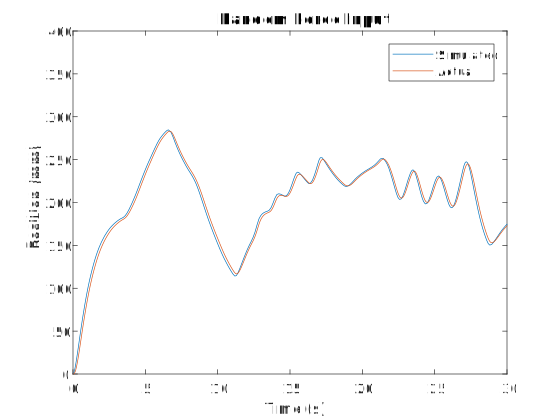
\includegraphics[width=0.9\linewidth]{Mar12_RandForce_Plot1}
	\caption{Admittance Verification with Interaction}
	\label{fig:VerInt}
\end{figure*}
	
	These tests confirm that the admittance controller adequately recreated the desired dynamics, and that the outer-loop PD controller tracked this behaviour. 
	
	\subsection{Verifying Haptic Control}
	
	\section{Healthy Subject Experiments}
	
\chapter{Conclusion}
	\section{Future Work}
	
	
\bibliography{thesis}
\bibliographystyle{ieeetr}
\end{document}